\chapter{Reference Client Unified}
\label{chap:reference-client-unified}

\section{Introduction}
Le projet Reference Client Unified (RCU) a pour objectif de créer une base de données client unifiée pour AmiParis afin d'améliorer l'expérience client, la gestion des relations client et l'efficacité des opérations commerciales. Cette solution centralisée intègre les données clients provenant de diverses sources comme Shopify et Cegid Y2, élimine les doublons et crée une vue complète de chaque client.

\section{Architecture du système}

L'architecture du système RCU est conçue pour intégrer efficacement des données provenant de multiples sources tout en garantissant la qualité et la cohérence des données.

\begin{figure}[H]
    \centering
    \includegraphics[width=1.0\textwidth]{images/system_architecture}
    \caption{Architecture globale du système RCU}
    \label{fig:system-architecture}
\end{figure}

L'architecture présentée dans la figure \ref{fig:system-architecture} montre les différentes couches du système:
\begin{itemize}
    \item \textbf{Systèmes externes}: Shopify (e-commerce), Cegid Y2 (point de vente) et formulaires web
    \item \textbf{Couche d'intégration}: Webhooks, API par lots et connecteurs personnalisés
    \item \textbf{Plateforme centrale}: Traitement des données, gestion des doublons, interface utilisateur et rapports
    \item \textbf{Stockage de données}: Base de données Salesforce et objets volumineux pour les grands ensembles de données
    \item \textbf{Intégrations externes}: Marketing Cloud et Power BI pour l'analyse
\end{itemize}

\subsection{Modèle de données}

Le modèle de données du système RCU est centré sur l'entité Account (Client) avec plusieurs objets connexes pour stocker les informations client complètes.

\begin{figure}[H]
    \centering
    \includegraphics[width=1.0\textwidth]{images/data_model_overview}
    \caption{Modèle de données RCU}
    \label{fig:data-model}
\end{figure}

La figure \ref{fig:data-model} présente les principales entités du modèle de données:
\begin{itemize}
    \item \textbf{Account}: Entité principale représentant un client unifié
    \item \textbf{Contact}: Informations de contact associées à un compte
    \item \textbf{ExternalSourceLink\_\_c}: Liens vers les systèmes sources externes
    \item \textbf{ConsentRecord\_\_c}: Enregistrements de consentement RGPD
    \item \textbf{Order\_\_c}: Commandes associées à un compte
    \item \textbf{OrderItem\_\_c}: Articles de commande individuels
    \item \textbf{Store\_\_c}: Magasins où les clients effectuent des achats
\end{itemize}

\section{Intégration des données}

\subsection{Webhooks pour l'intégration en temps réel}

Pour assurer une intégration efficace et en temps réel des données client, le système utilise des webhooks qui permettent de capturer les événements importants des systèmes sources.

\begin{figure}[H]
    \centering
    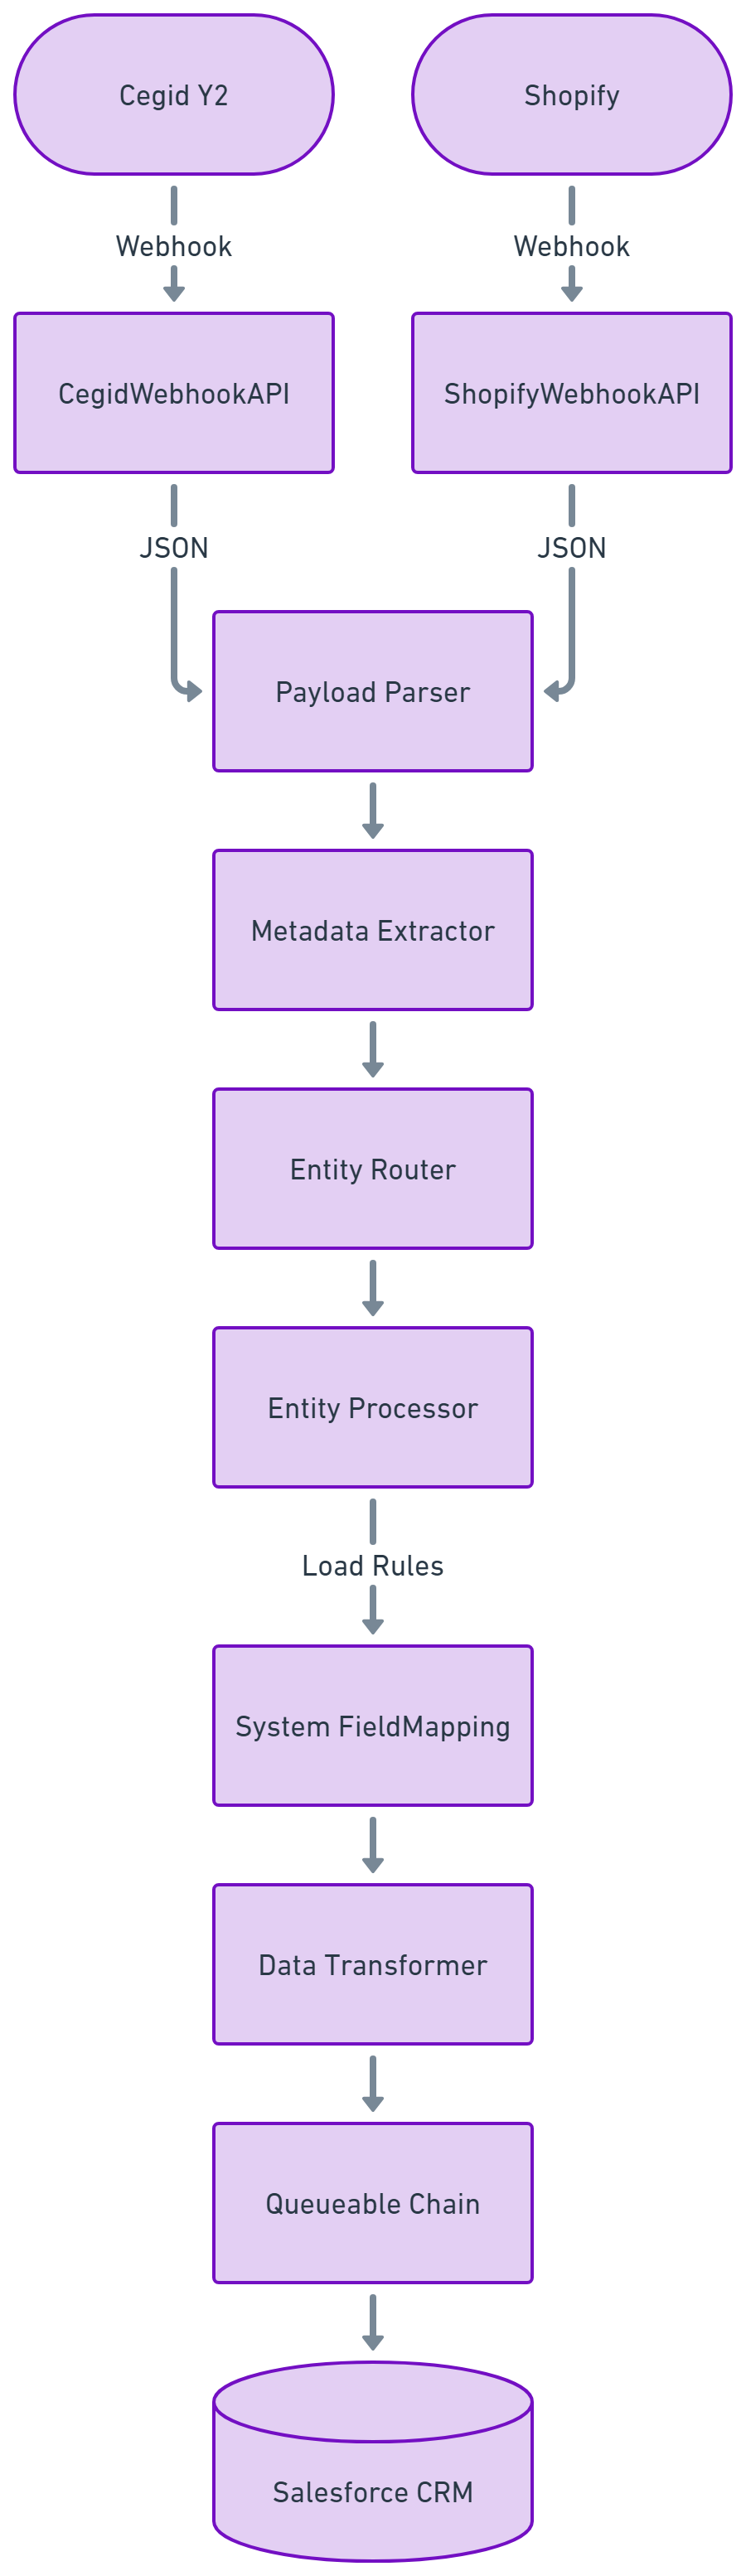
\includegraphics[width=1.0\textwidth]{images/webhook_architecture}
    \caption{Architecture des webhooks pour l'intégration des données}
    \label{fig:webhook-architecture}
\end{figure}

Comme illustré dans la figure \ref{fig:webhook-architecture}, les événements sont capturés par les systèmes sources (Shopify, Cegid Y2) et envoyés à Salesforce où ils sont traités en suivant un processus standardisé. Cette approche permet une mise à jour quasi instantanée des données client dans le système RCU.

\subsection{Transformation des données}

La transformation des données est une étape cruciale pour standardiser les informations provenant de sources hétérogènes.

\begin{figure}[H]
    \centering
    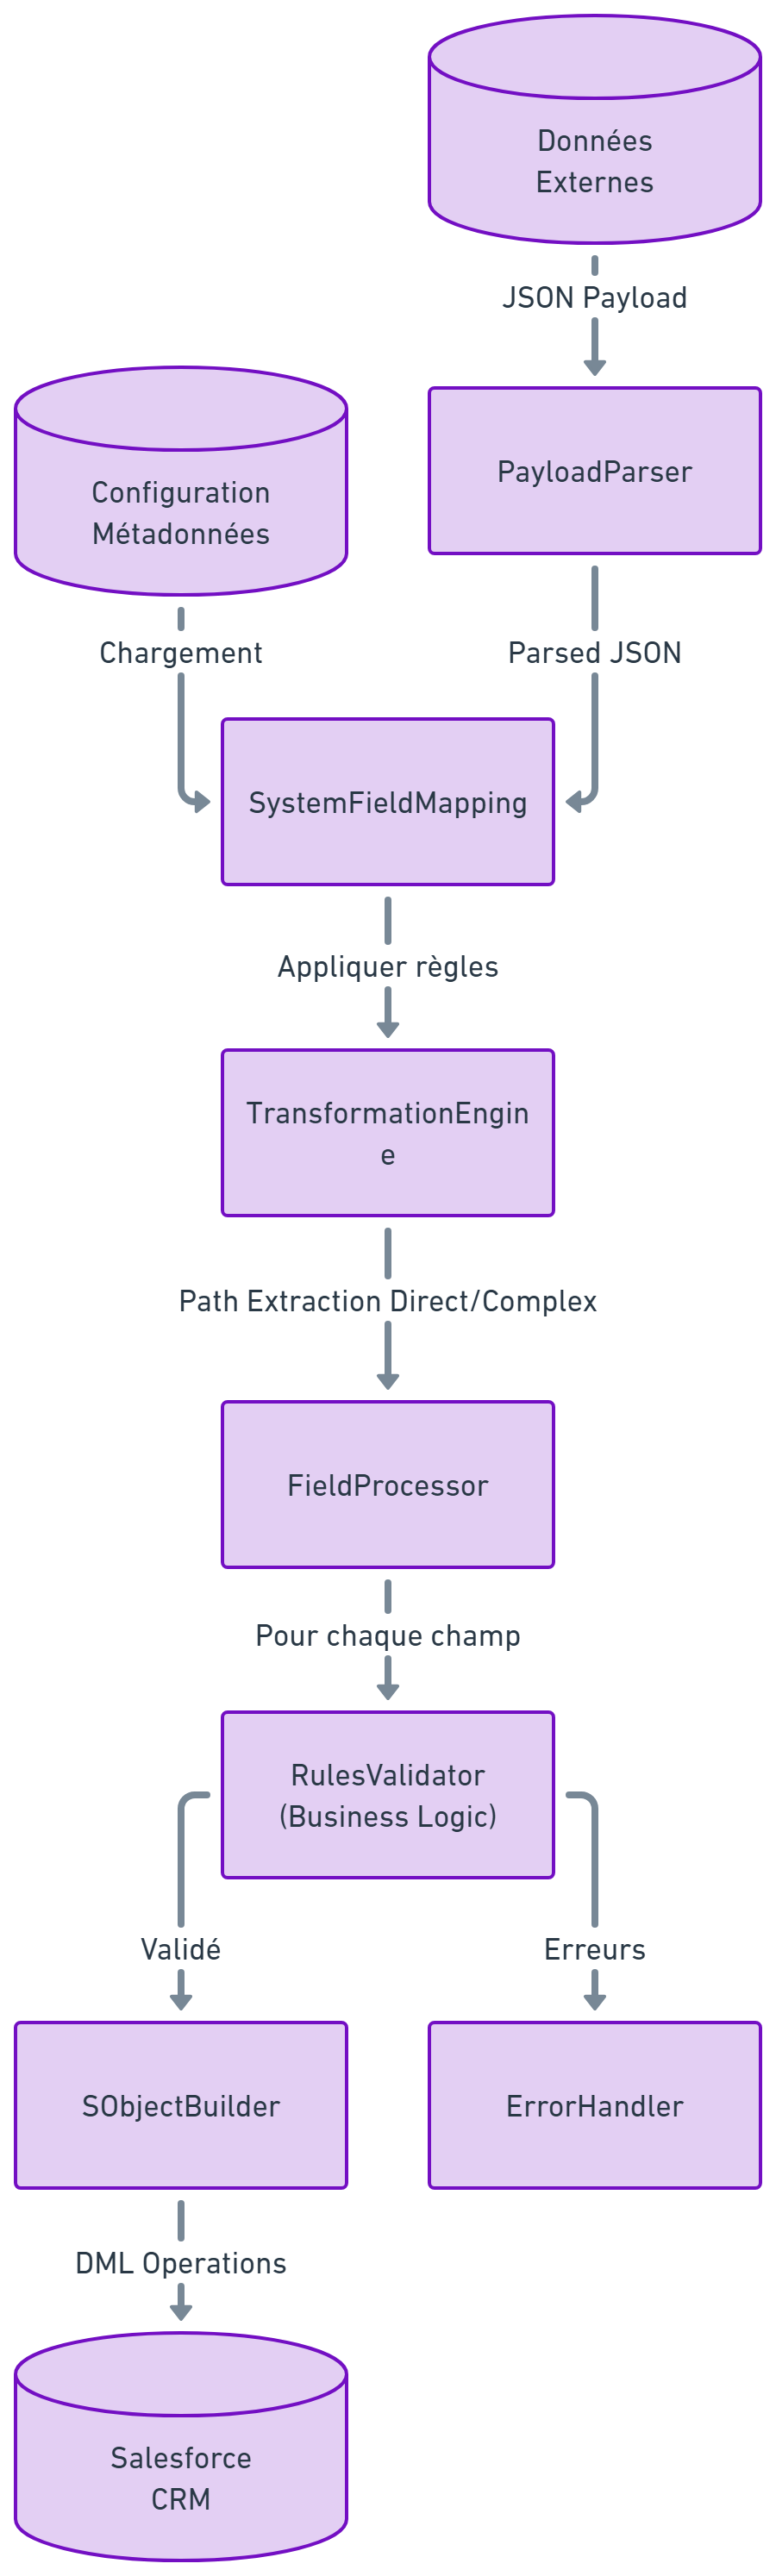
\includegraphics[width=0.9\textwidth]{images/data_transformation}
    \caption{Processus de transformation des données}
    \label{fig:data-transformation}
\end{figure}

Le processus illustré dans la figure \ref{fig:data-transformation} montre comment les données brutes sont transformées grâce à la configuration SystemFieldMapping. Cette configuration permet de définir des règles de transformation spécifiques pour chaque champ.

\subsection{Configuration de SystemFieldMapping}

La table \ref{tab:system-field-mapping} présente les différentes logiques de transformation utilisées dans le système.

\begin{table}[H]
\centering
\caption{Configuration de SystemFieldMapping}
\label{tab:system-field-mapping}
\begin{tabularx}{\textwidth}{|X|X|X|X|}
\hline
\textbf{Type de logique} & \textbf{Description} & \textbf{Champ source} & \textbf{Champ cible} \\
\hline
DirectMapping & Copie directe sans modification & FirstName & FirstName \\
\hline
ConvertToLowerCase & Conversion en minuscules & Email & Email \\
\hline
DateIso & Conversion de format de date & OrderDate & OrderDate \\
\hline
PhoneFormat & Standardisation des numéros de téléphone & Phone & Phone \\
\hline
Concatenate & Fusion de plusieurs champs & FirstName + LastName & FullName \\
\hline
CustomLogic & Logique personnalisée via APEX & Various & Status \\
\hline
\end{tabularx}
\end{table}

\section{Gestion des doublons}

La détection et la gestion des doublons sont des fonctionnalités essentielles du système RCU pour maintenir une vue client unifiée.

\begin{figure}[H]
    \centering
    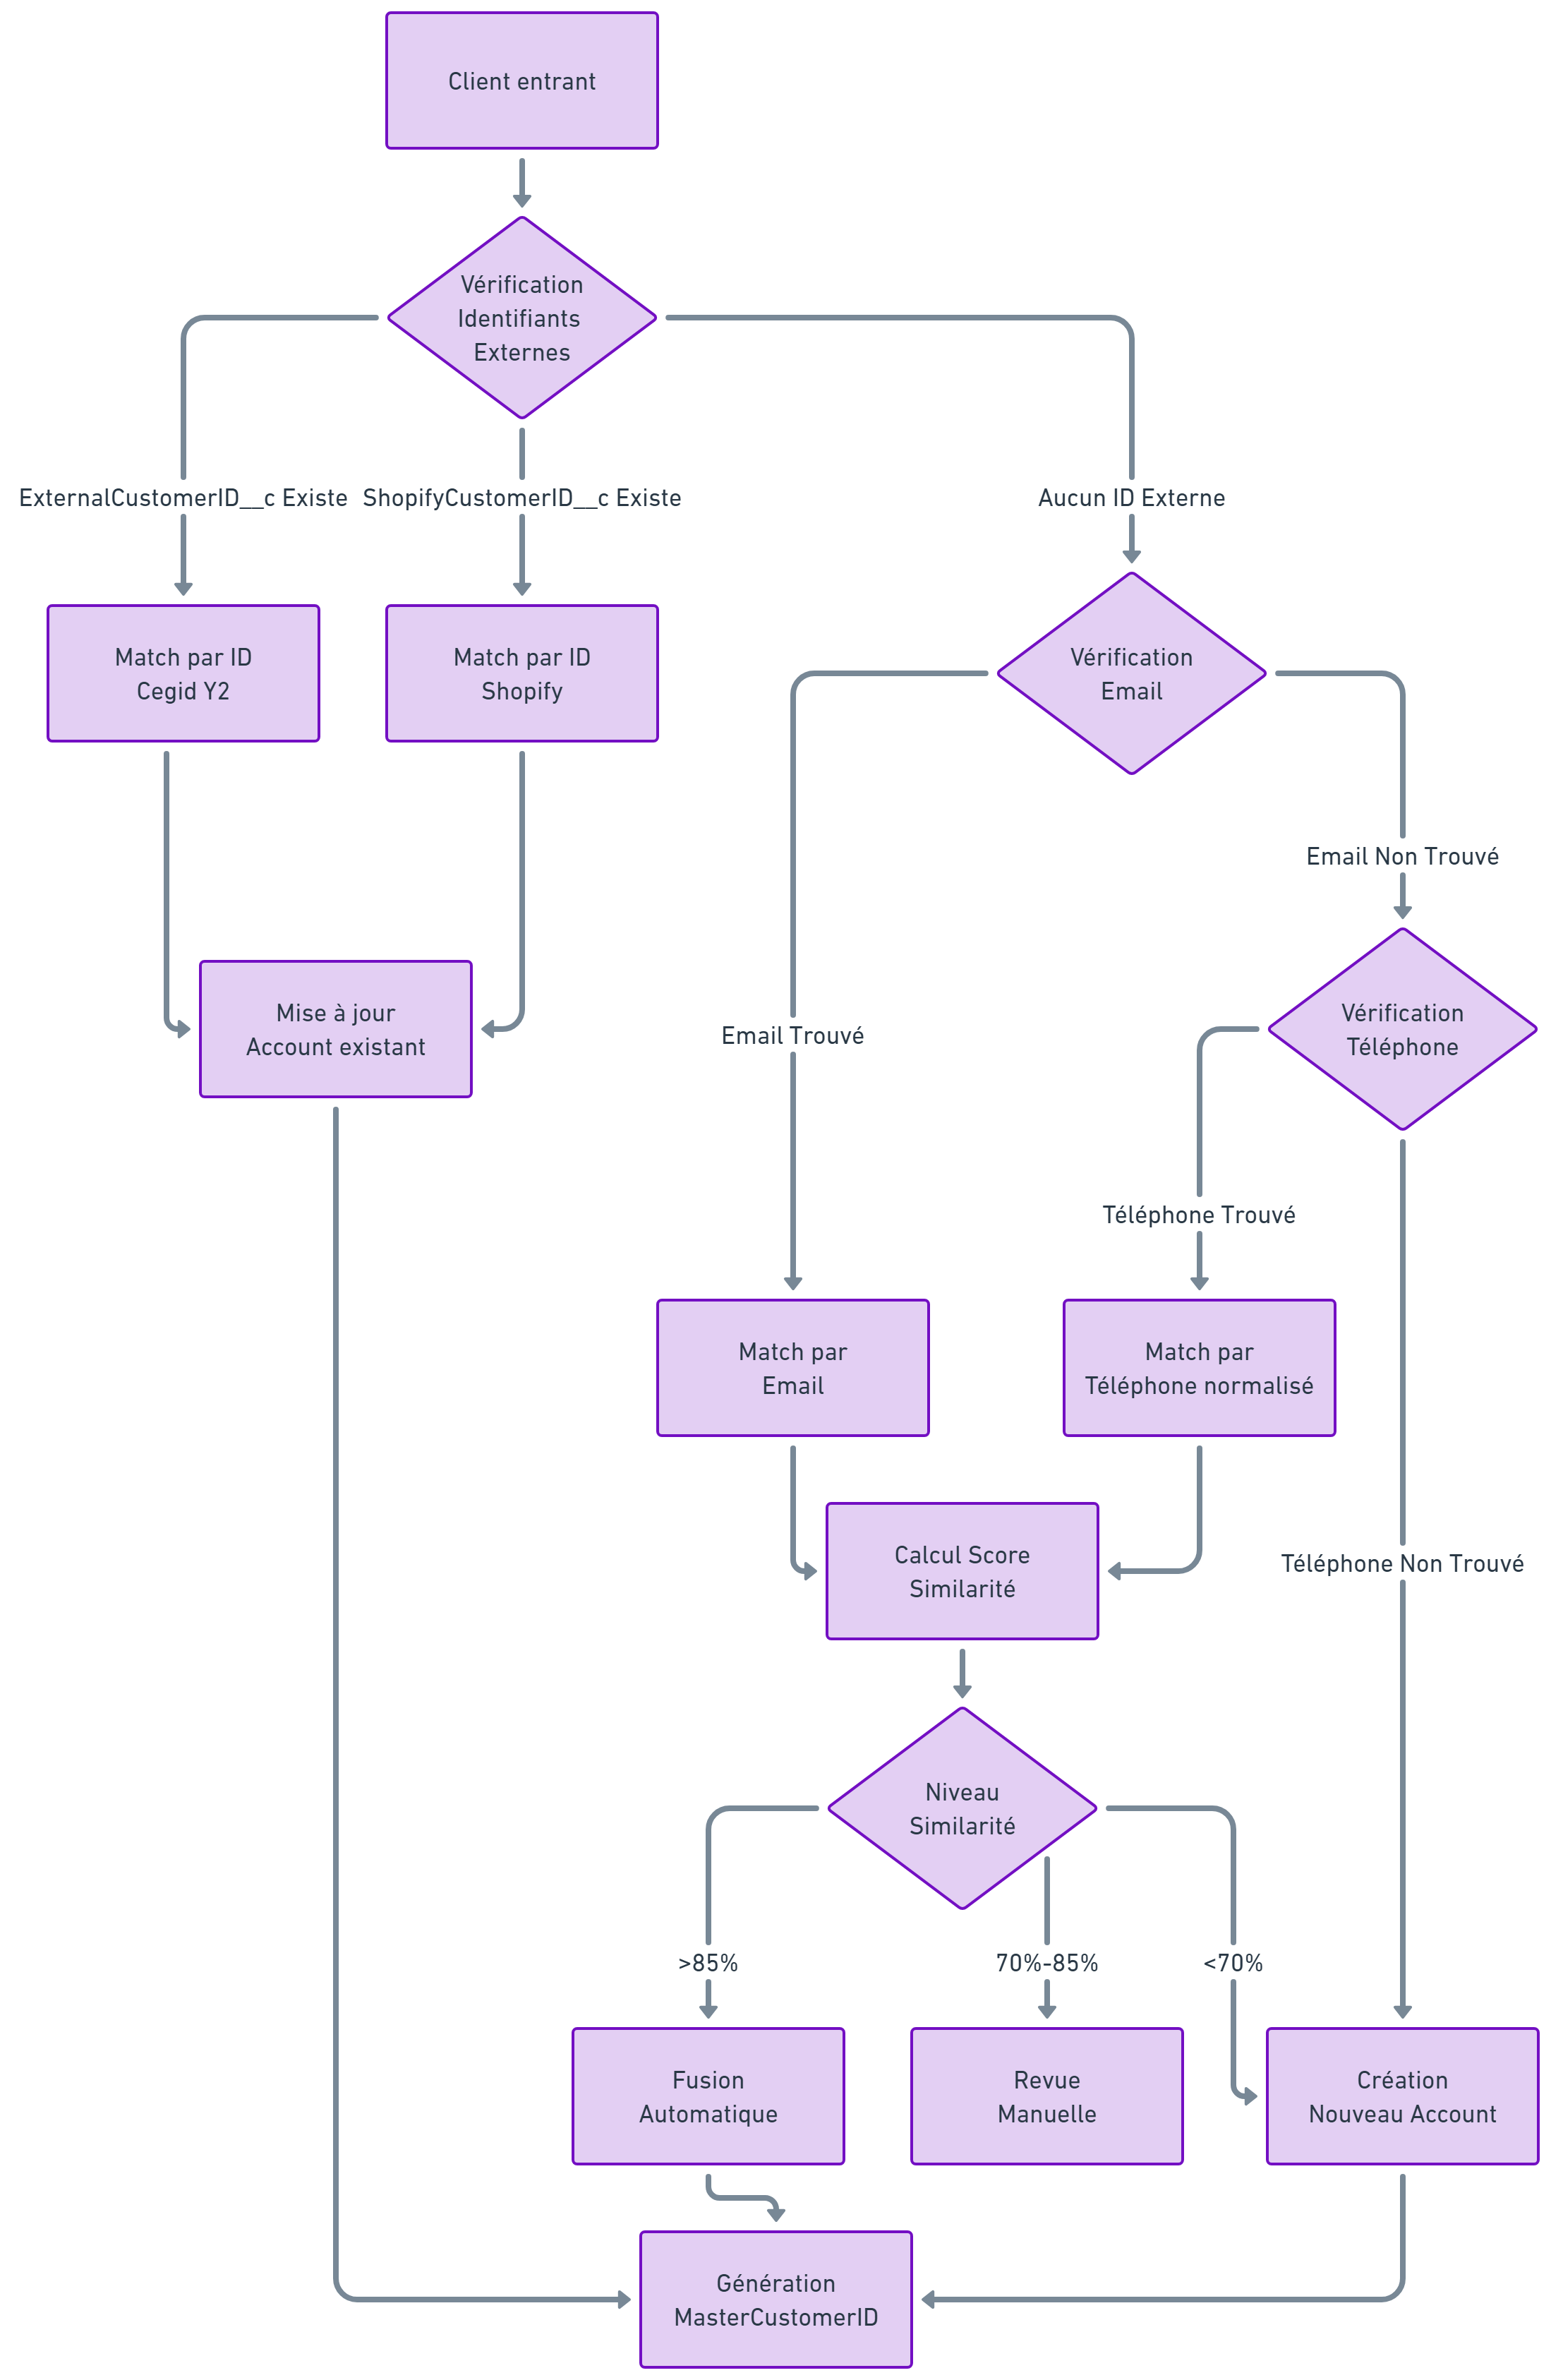
\includegraphics[width=0.95\textwidth]{images/deduplication_strategy}
    \caption{Stratégie de déduplication}
    \label{fig:dedup-strategy}
\end{figure}

La figure \ref{fig:dedup-strategy} illustre le processus de déduplication qui compare les enregistrements entrants avec les enregistrements existants pour identifier et gérer les doublons potentiels.

\subsection{Logique de déduplication dans AccountTriggerHandler}

Le déclencheur de compte joue un rôle central dans la gestion des doublons en implémentant une logique sophistiquée pour la détection et la fusion des comptes clients.

\begin{figure}[H]
    \centering
    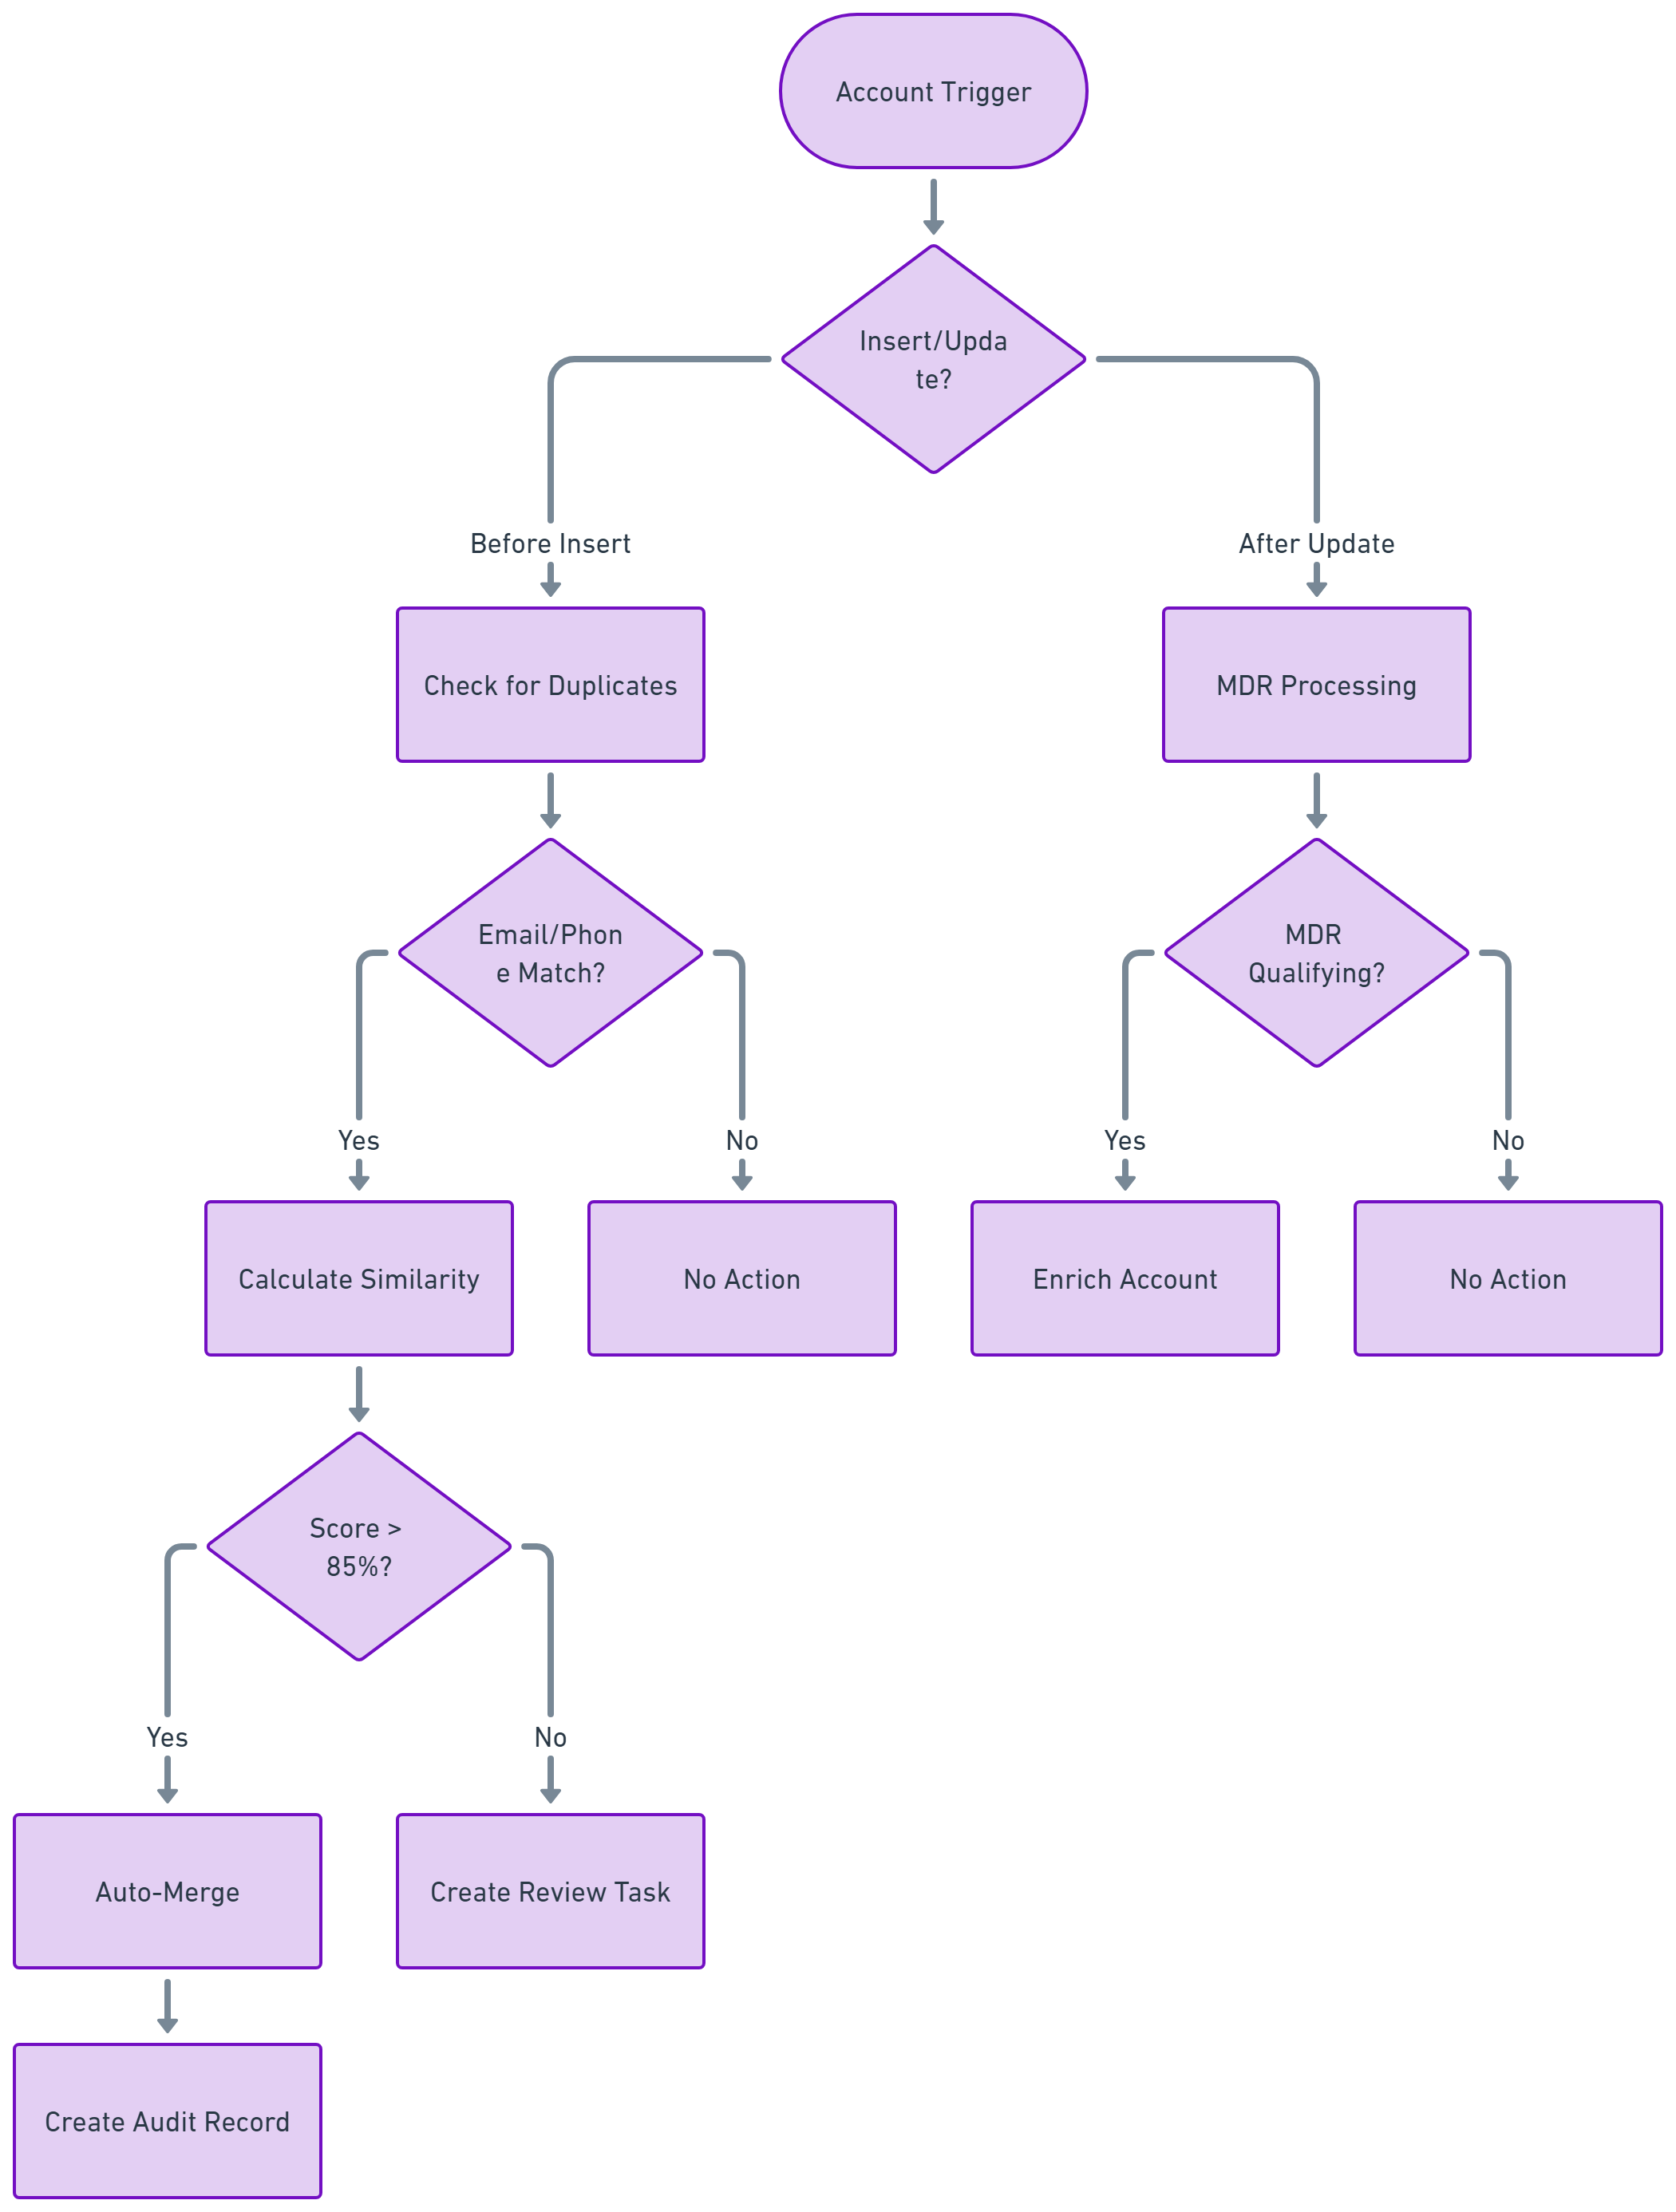
\includegraphics[width=0.95\textwidth]{images/account_trigger_handler}
    \caption{Processus de gestion des doublons dans AccountTriggerHandler}
    \label{fig:account-trigger}
\end{figure}

La figure \ref{fig:account-trigger} détaille le flux de travail du déclencheur de compte, qui comprend:
\begin{itemize}
    \item Détection des doublons potentiels lors de l'insertion ou la mise à jour
    \item Vérification des correspondances par email ou téléphone
    \item Calcul d'un score de similarité entre les enregistrements
    \item Fusion automatique ou création d'une tâche de révision selon le score
    \item Enregistrement des actions de fusion pour l'audit
\end{itemize}

\section{Traitement asynchrone des données}

Pour gérer efficacement de grands volumes de données sans impacter les performances du système, le RCU utilise des traitements asynchrones.

\begin{figure}[H]
    \centering
    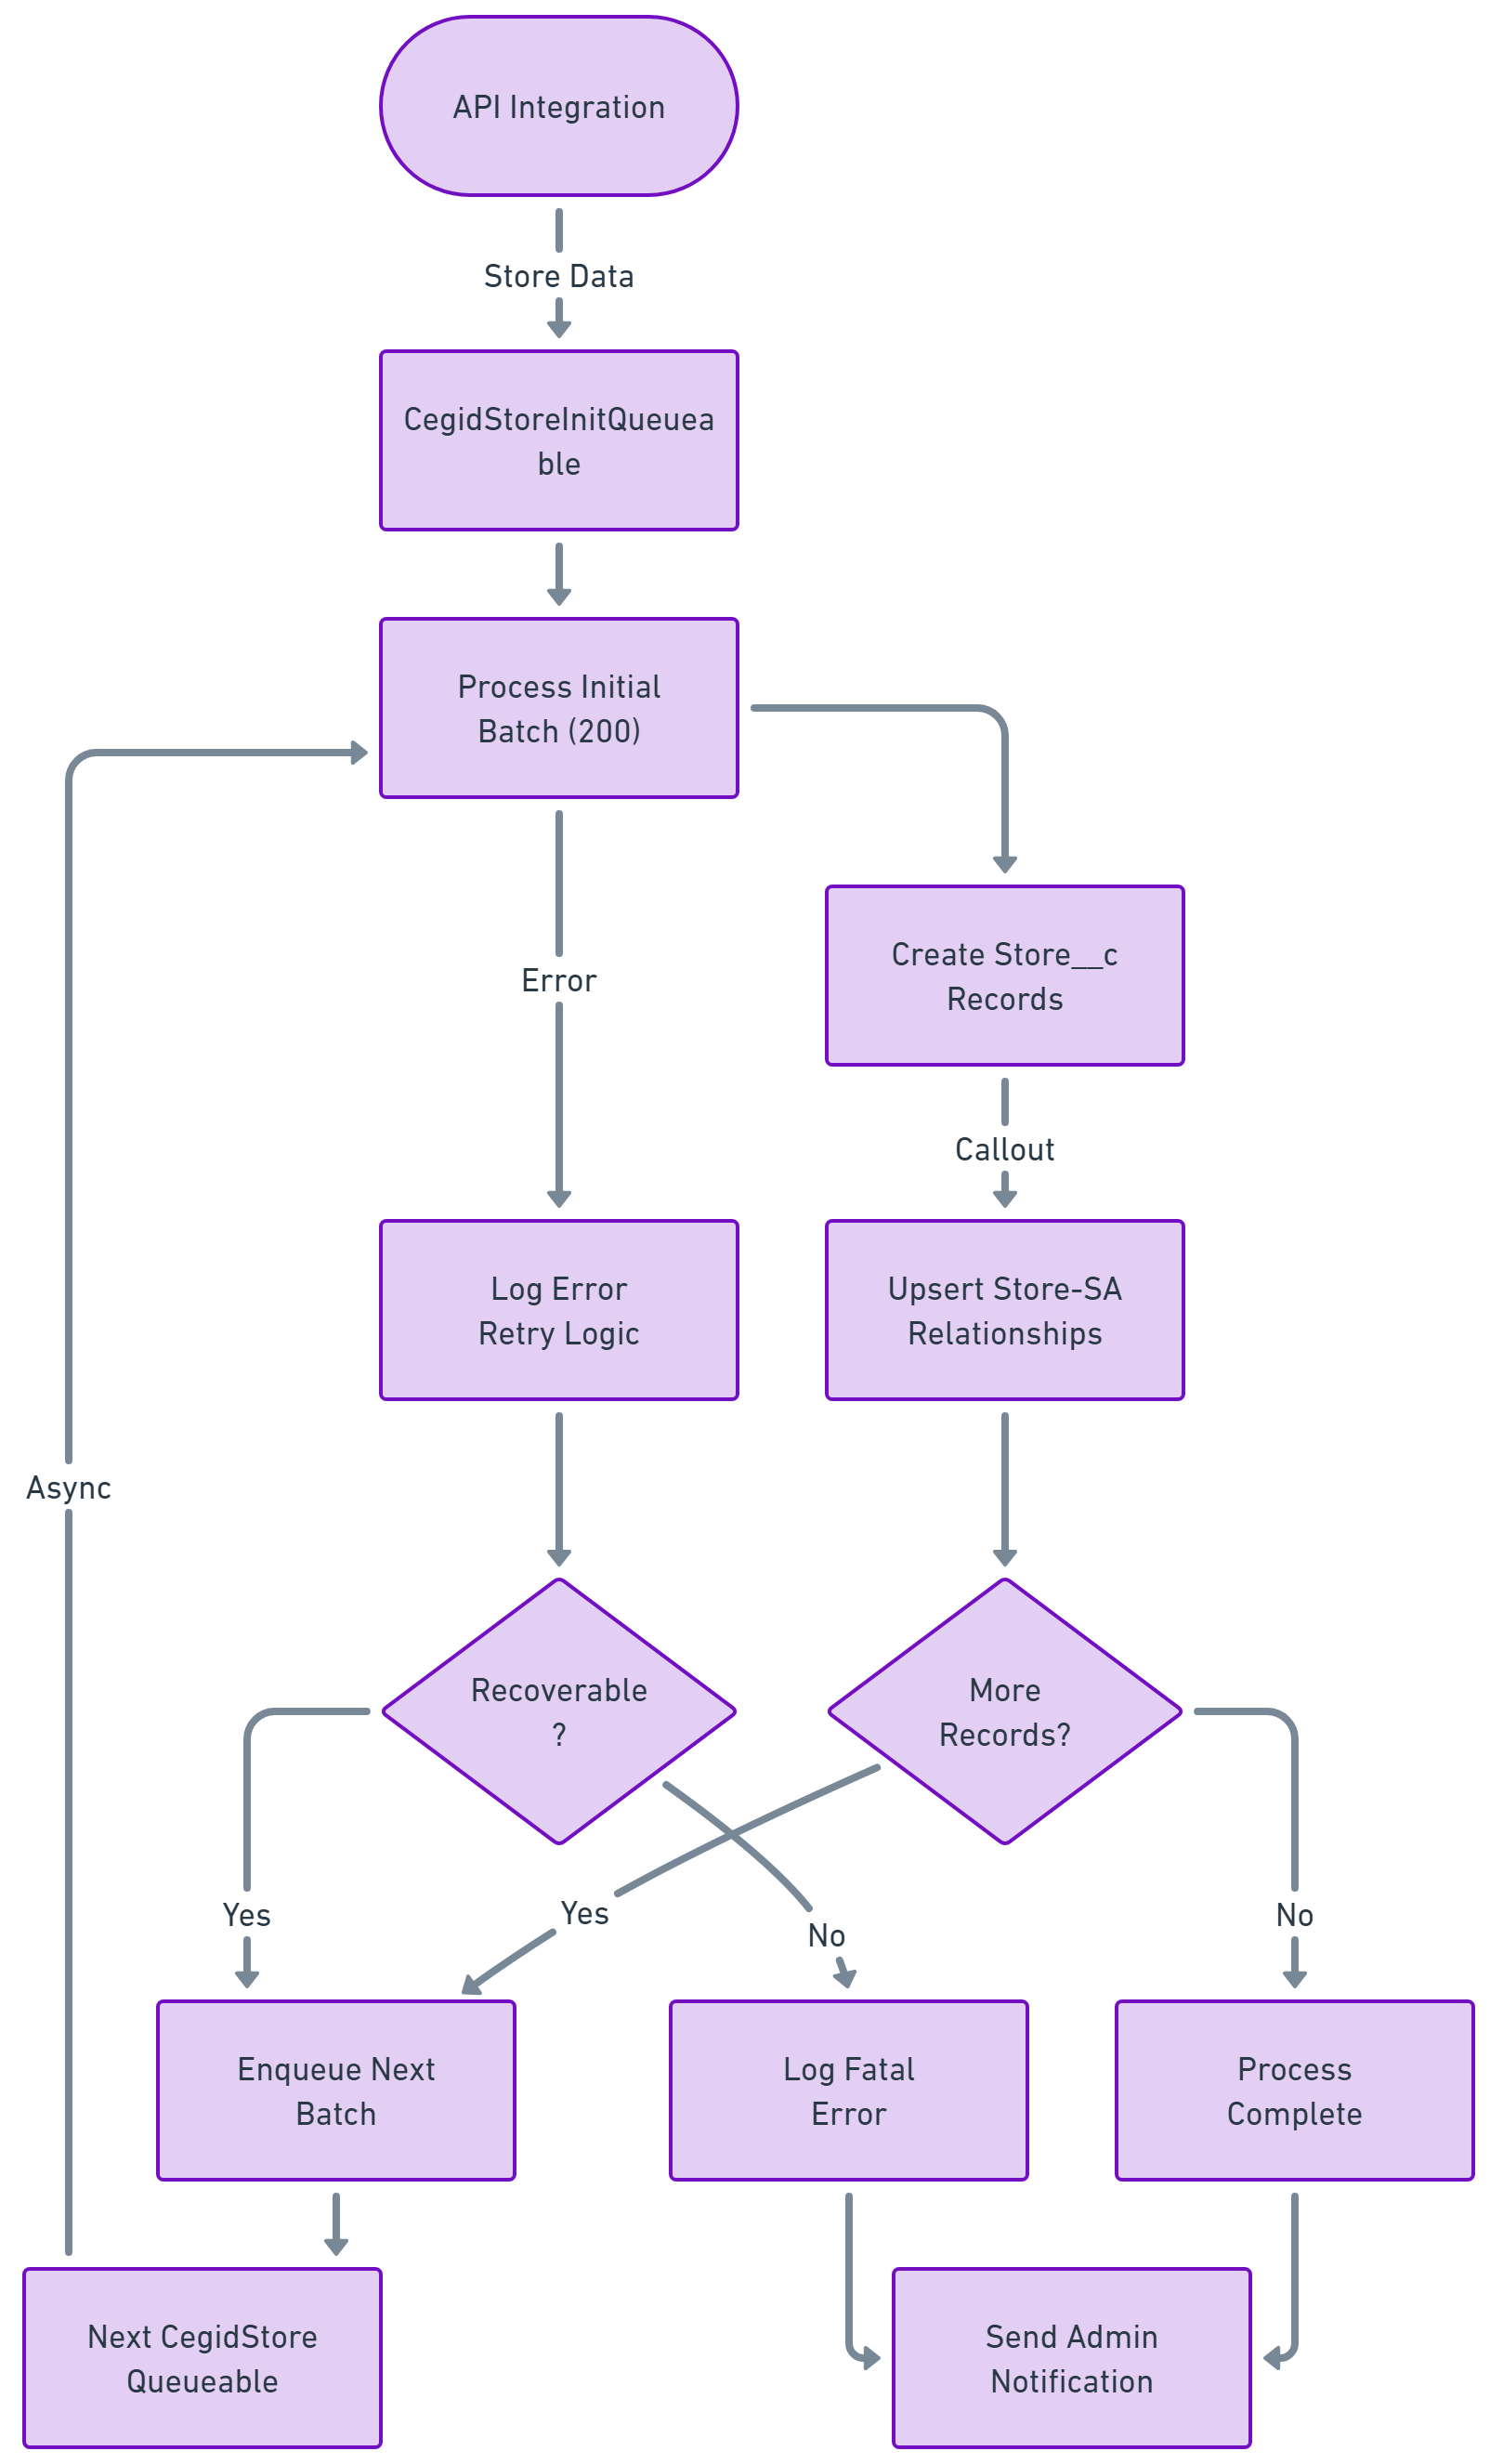
\includegraphics[width=0.95\textwidth]{chapters/images/cegid_store_init_queueable}
    \caption{Traitement asynchrone avec CegidStoreInitQueueable}
    \label{fig:queueable}
\end{figure}

La figure \ref{fig:queueable} montre le fonctionnement de la classe CegidStoreInitQueueable, qui:
\begin{itemize}
    \item Traite des lots de 200 enregistrements à la fois
    \item Crée des enregistrements Store\_\_c dans Salesforce
    \item Établit des relations entre les magasins et les comptes associés
    \item Enchaîne les traitements asynchrones pour gérer de grands volumes
    \item Intègre une gestion des erreurs avec possibilité de reprise
\end{itemize}

\section{Gestion du consentement RGPD}

La conformité au RGPD est un aspect crucial du système RCU, avec une attention particulière portée à la gestion du consentement client.

\begin{figure}[H]
    \centering
    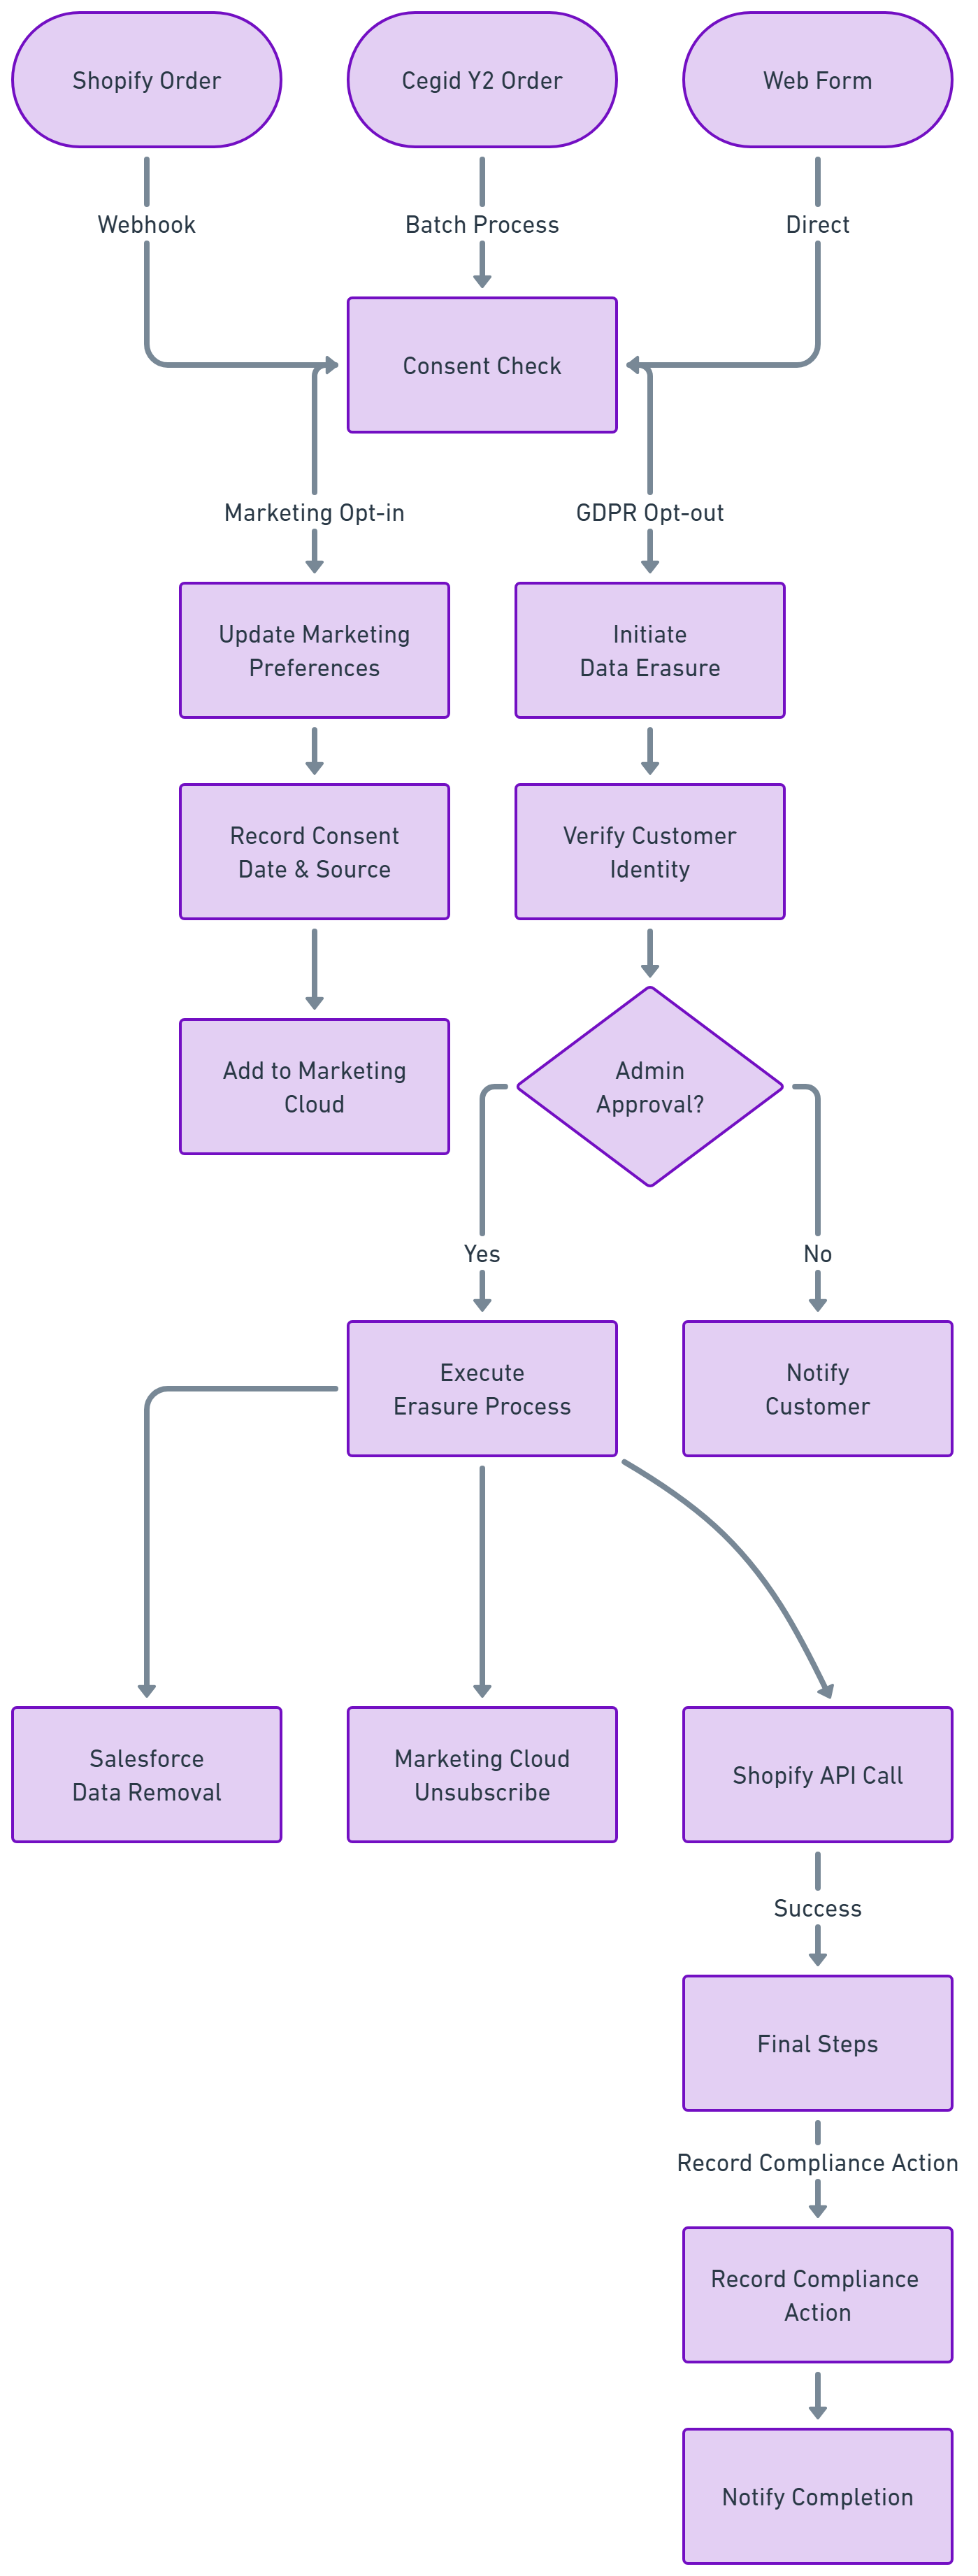
\includegraphics[width=1.0\textwidth]{chapters/images/gdpr_consent_flow}
    \caption{Flux de gestion du consentement RGPD}
    \label{fig:gdpr-consent}
\end{figure}

La figure \ref{fig:gdpr-consent} illustre le flux de traitement du consentement client, incluant:
\begin{itemize}
    \item Différentes sources de consentement (commandes Shopify, Cegid, formulaires web)
    \item Vérification et enregistrement des préférences marketing
    \item Processus de gestion des demandes d'effacement des données
    \item Approbation administrative pour les effacements
    \item Suppression coordonnée des données dans tous les systèmes intégrés
    \item Enregistrement des actions pour la conformité réglementaire
\end{itemize}

\section{Conclusion}

Le système Reference Client Unified (RCU) offre à AmiParis une solution robuste pour créer et maintenir une vue client unifiée. Grâce à son architecture modulaire, ses processus d'intégration en temps réel, ses mécanismes de déduplication avancés et sa gestion rigoureuse du consentement RGPD, le système permet d'améliorer significativement la qualité des données client et l'efficacité des opérations commerciales. La centralisation des données client constitue une base solide pour les initiatives futures d'analyse des données, de personnalisation de l'expérience client et d'optimisation des campagnes marketing. 